\chapter{Scenario Implementation and Results}
% Introduction
This chapter presents results of two scenarios using the proposed navigation filter and its underlying components discussed in previous chapters. Both scenarios use a similar trajectory and will be discussed thoroughly to avoid confusion. First, the chapter starts with a discussion of the first scenario and the five separate cases run in Monte-Carlo for scenario one. Following a description of scenario one, results from specific cases will be presented, highlighting the strong and weak points of the proposed navigation filter. The results from the remaining cases not presented in this chapter can be found in the appendix of this work. Once the analysis of scenario one has concluded, a description of scenario two is presented, followed by Monte-Carlo statistical analyses. The performance of the proposed navigation filter will be determined based on 100-run Monte-Carlo simulations each scenario and and each case. As a visual comparison, a loosely-coupled IMU is added for the same scenarios.
\section{\textbf{Simulated Trajectory}}
As stated previously, both scenarios one and two will be flying a similar trajectory. This trajectory meets the observability criteria discussed in Chapter 5, featuring continuous banking of the aircraft with a steady climb to provide excitation to the angular states for better estimates of the orientation during simulations. Figure~\ref{fig:trajectory} presents the \textit{S}-like trajectory and Table~\ref{tbl:trajectory} presents the initial conditions of the simulated Diamond DA-40.

\begin{figure}[!ht]
    \centering
    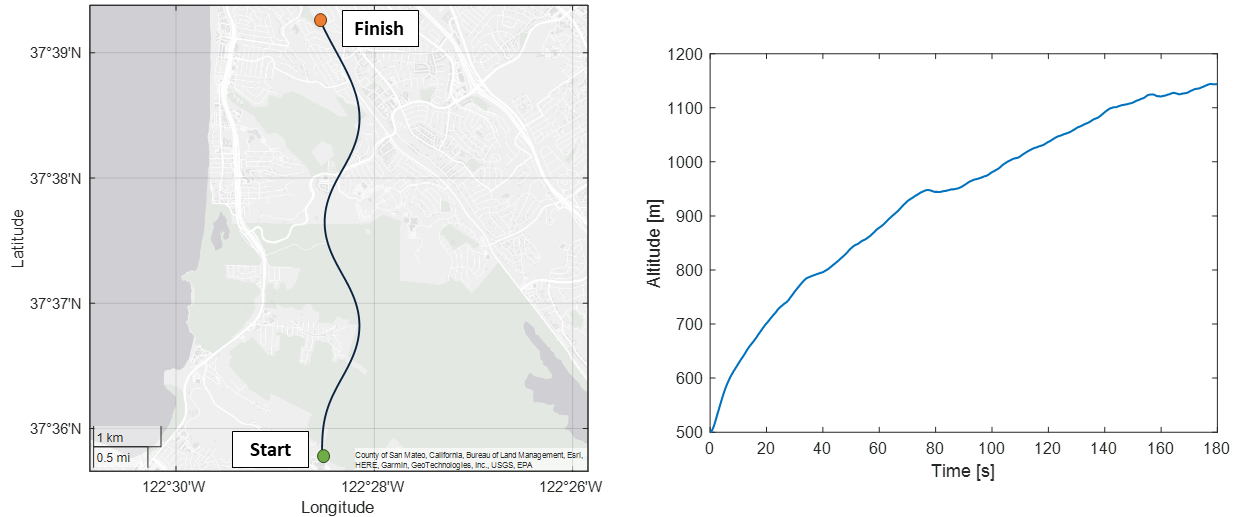
\includegraphics[width=\linewidth]{Figures/trajectoryfigure.png}
    \caption{Simulated trajectory for both presented scenarios with accompanying altitude flightpath. }\label{fig:trajectory}
\end{figure}

\begin{table}[!ht]
    \caption{Initial conditions for simulated trajectory from Figure~\ref{fig:trajectory}.}\label{tbl:trajectory}
    \centering
    \begin{tabular}{lcc}
        \toprule
        \textbf{Condition}       & \textbf{Value}                                      & \textbf{Units}                     \\
        \midrule
        Date                     & June 15, 2022                                       & \textit{DateTime} Object           \\
        Duration                 & 180                                                 & \(s\)                              \\
        Monte-Carlo Runs         & 100                                                 & {--}                               \\
        Frequency                & 200                                                 & Hz                                 \\
        Trajectory               & \textit{SCurveFlightPath.mat}                       & See Chapter 5                      \\
        Velocity Disturbance     & \(\left[300, \; 300, \; 0\right]\)                  & \(m/s\)                            \\
        Angular Rate Disturbance & \(\left[10^{-12}, \; 10^{-12}, \; 10^{-12}\right]\) & \(rad/s\)                          \\
        Position Disturbance     & \(\left[0, \; 0, \; 10\right]\)                     & \(m\)                              \\
        Clock Type               & OCXO                                                & {--}                               \\
        Initial Velocity         & \(\left[75, \; 0, \; 0\right]\)                     & \(m/s\)                            \\
        Initial Angular Rate     & \(\left[0, \; 0, \; 0\right]\)                      & \(rad/s\)                          \\
        Initial Position         & \(\left[0.65617, \; -2.1376, \; 500\right]\)        & \(\left[rad, \; rad, \; m\right]\) \\
        Initial Attitude         & \(\left[0, \; 0, \; 0\right]\)                      & \(rad\)                            \\
        Initial Clock Terms      & \(\left[0, \; 0\right]\)                            & \(\left[m, \; m/s\right]\)         \\
        Channel \(C/N_0\)        & \(45\)                                              & db-Hz                              \\

        \bottomrule
    \end{tabular}
\end{table}

\section{\textbf{Scenario 1}}

\subsection{\textbf{Interference Overview}}

\begin{figure}[!ht]
    \centering
    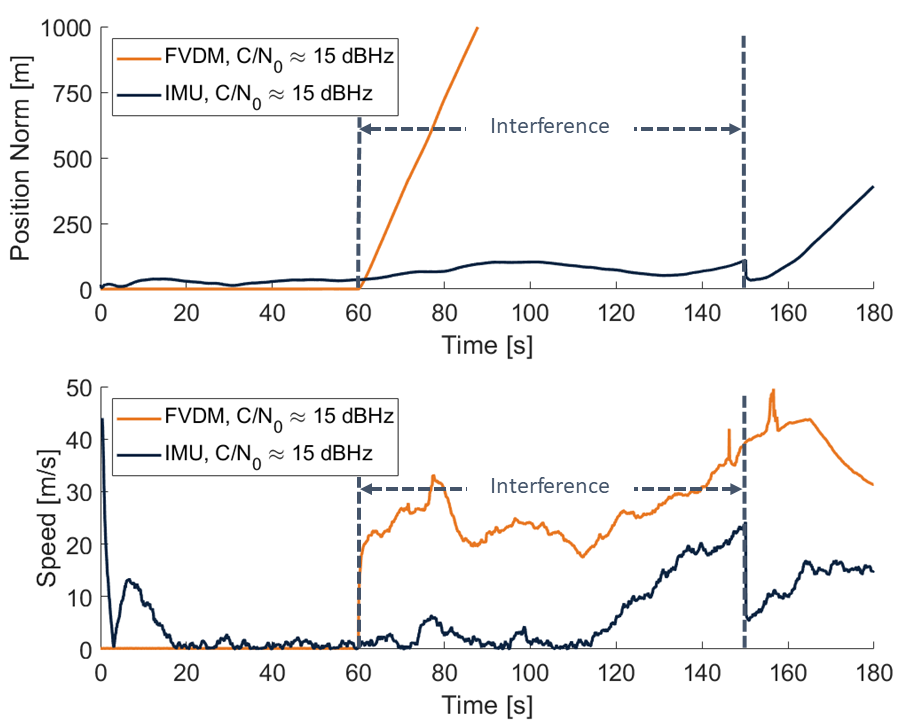
\includegraphics[width=0.75\linewidth]{Figures/Results/trajectoryfigure/Slide14.PNG}
    \caption{Position and speed estimates using the proposed navigation filter when subject to instantaneous interference, bringing the \(C/N_0\) to \(15\) dB-Hz.}\label{fig:PosVel15}
\end{figure}

\begin{figure}[!ht]
    \centering
    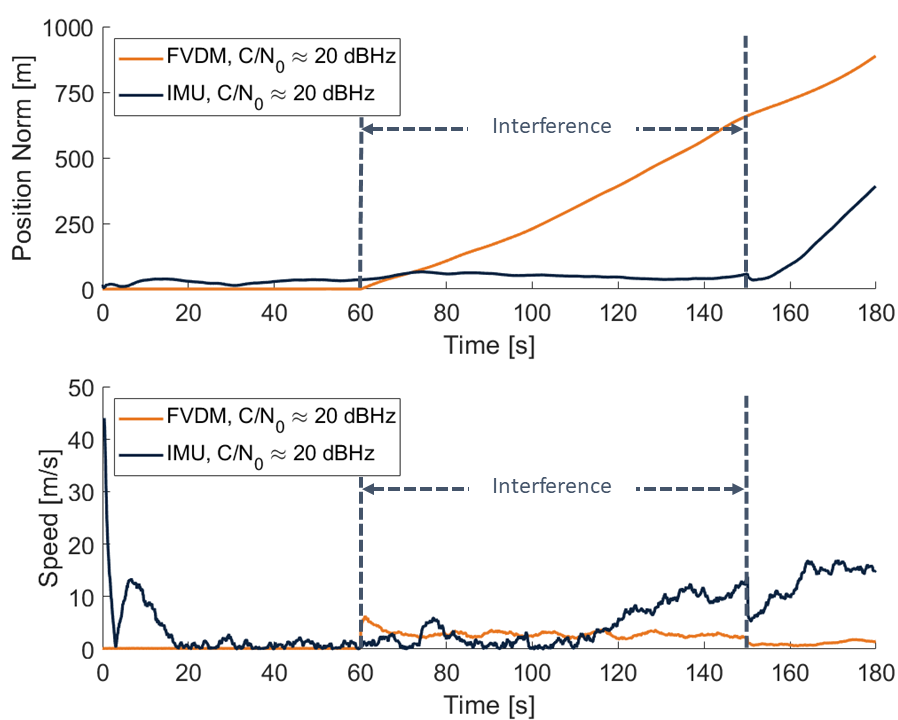
\includegraphics[width=0.75\linewidth]{Figures/Results/trajectoryfigure/Slide15.PNG}
    \caption{Position and speed estimates using the proposed navigation filter when subject to instantaneous interference, bringing the \(C/N_0\) to \(20\) dB-Hz.}\label{fig:PosVel20}
\end{figure}

\begin{figure}[!ht]
    \centering
    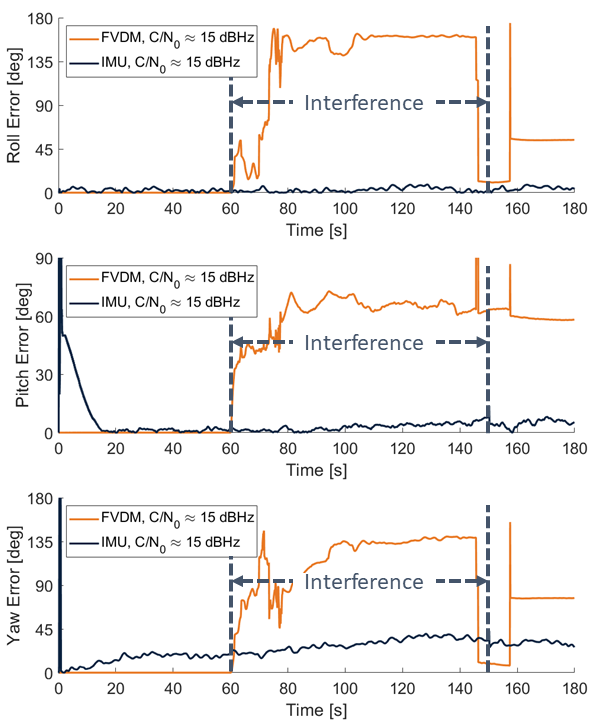
\includegraphics[width=0.75\linewidth]{Figures/Results/trajectoryfigure/Slide2.PNG}
    \caption{Euler attitude estimates using the proposed navigation filter when subject to instantaneous interference, bringing the \(C/N_0\) to \(15\) dB-Hz.}\label{fig:Eul15}
\end{figure}

\begin{figure}[!ht]
    \centering
    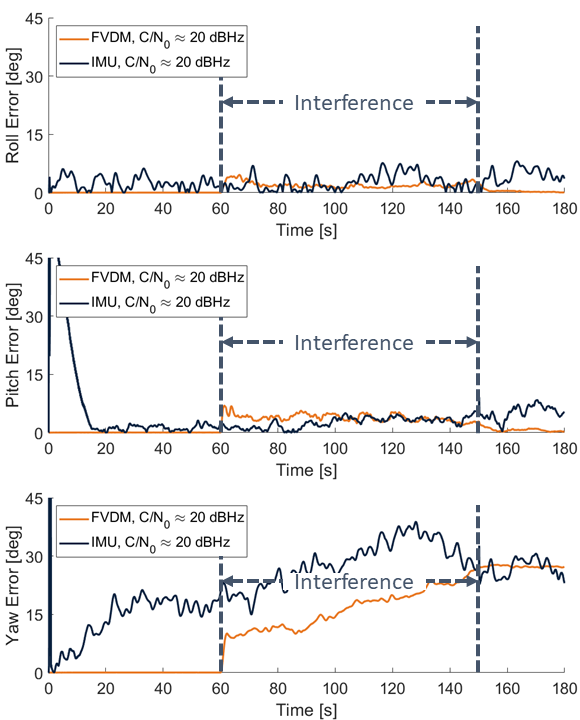
\includegraphics[width=0.75\linewidth]{Figures/Results/trajectoryfigure/Slide3.PNG}
    \caption{Euler attitude estimates using the proposed navigation filter when subject to instantaneous interference, bringing the \(C/N_0\) to \(20\) dB-Hz.}\label{fig:Eul20}
\end{figure}

\begin{figure}[!ht]
    \centering
    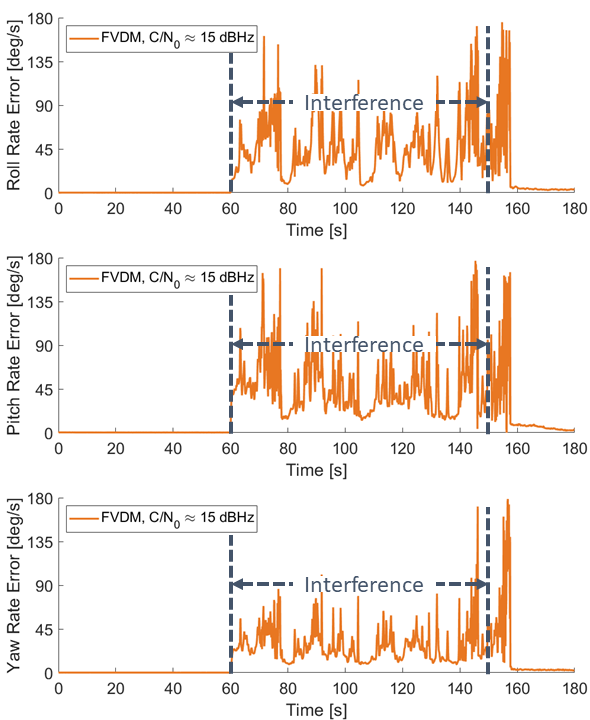
\includegraphics[width=0.75\linewidth]{Figures/Results/trajectoryfigure/Slide8.PNG}
    \caption{Angular rate estimates using the proposed navigation filter when subject to instantaneous interference, bringing the \(C/N_0\) to \(15\) dB-Hz.}\label{fig:Ang15}
\end{figure}

\begin{figure}[!ht]
    \centering
    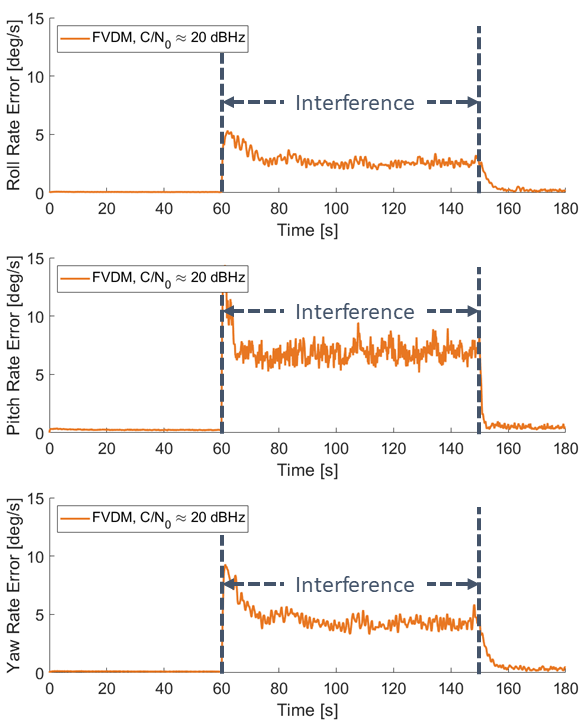
\includegraphics[width=0.75\linewidth]{Figures/Results/trajectoryfigure/Slide9.PNG}
    \caption{Angular rate estimates using the proposed navigation filter when subject to instantaneous interference, bringing the \(C/N_0\) to \(20\) dB-Hz.}\label{fig:Ang20}
\end{figure}

\begin{figure}[!ht]
    \centering
    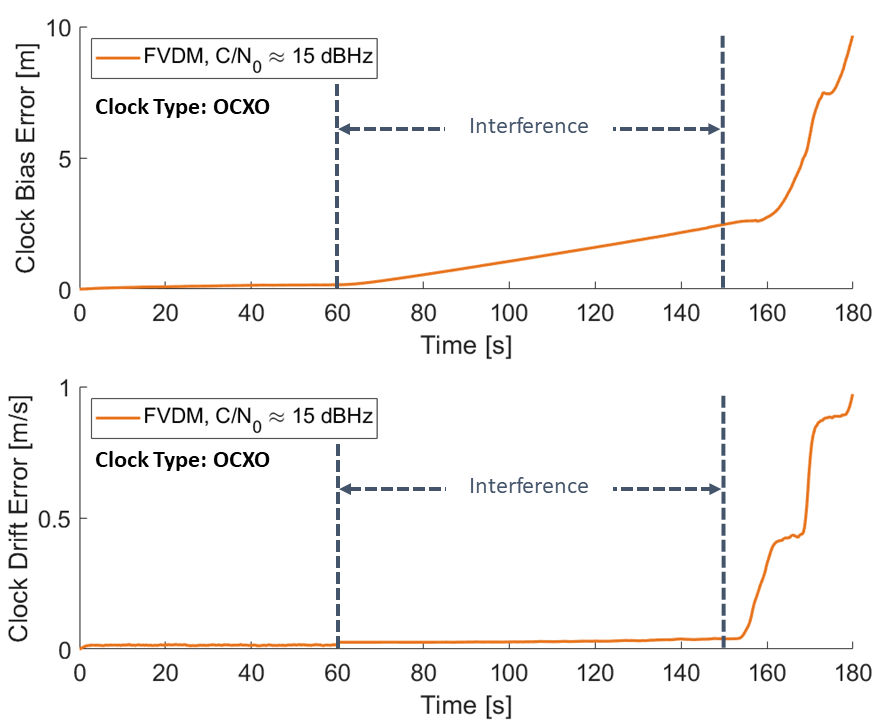
\includegraphics[width=0.75\linewidth]{Figures/Results/trajectoryfigure/Slide20.PNG}
    \caption{Clock bias and Clock drift estimates using the proposed navigation filter when subject to instantaneous interference, bringing the \(C/N_0\) to \(15\) dB-Hz.}\label{fig:Clk15}
\end{figure}

\begin{figure}[!ht]
    \centering
    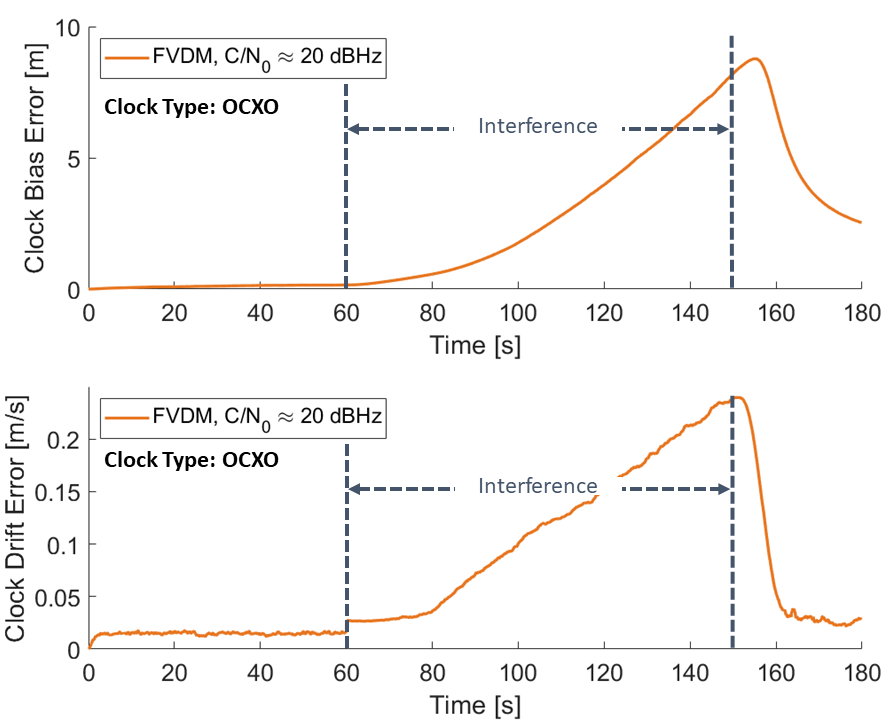
\includegraphics[width=0.75\linewidth]{Figures/Results/trajectoryfigure/Slide21.PNG}
    \caption{Clock bias and Clock drift estimates using the proposed navigation filter when subject to instantaneous interference, bringing the \(C/N_0\) to \(20\) dB-Hz.}\label{fig:Clk20}
\end{figure}

\section{\textbf{Scenario 2}}

\subsection{\textbf{Interference Overview}}

\begin{figure}[!ht]
    \centering
    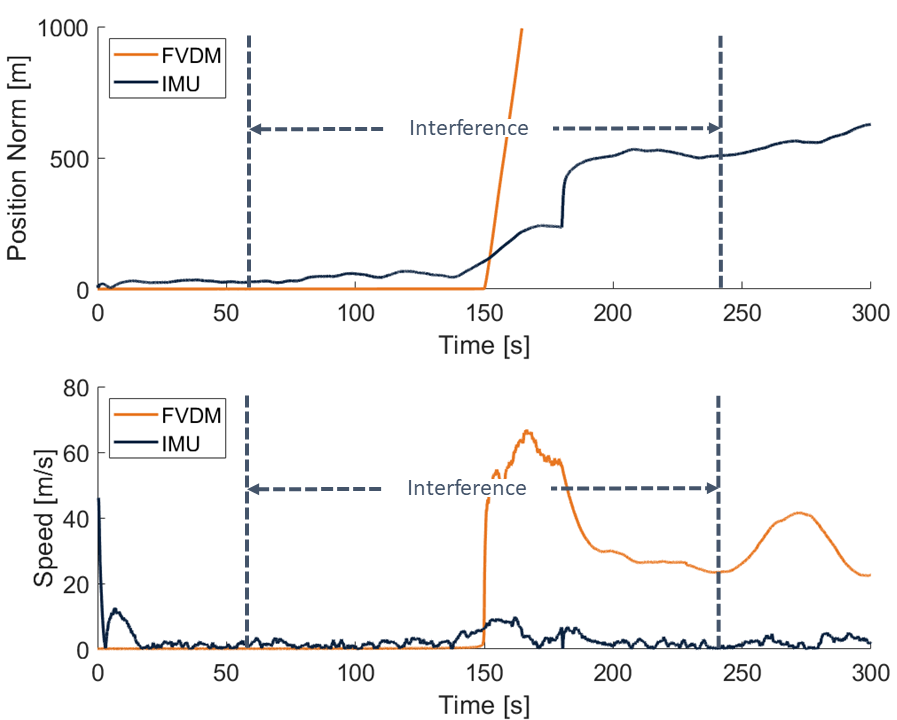
\includegraphics[width=0.75\linewidth]{Figures/Results/trajectoryfigure/Slide19.PNG}
    \caption{Position and speed estimates using the proposed navigation filter when subject to interference that grows stronger as the flight vehicles travels closer to the emitter.}\label{fig:PosVelScene2}
\end{figure}


\begin{figure}[!ht]
    \centering
    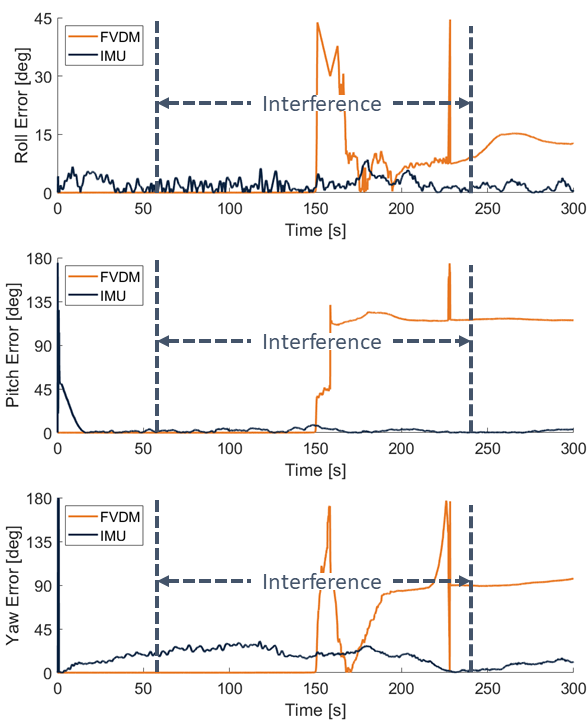
\includegraphics[width=0.75\linewidth]{Figures/Results/trajectoryfigure/Slide7.PNG}
    \caption{Position and speed estimates using the proposed navigation filter when subject to interference that grows stronger as the flight vehicles travels closer to the emitter.}\label{fig:EulScene2}
\end{figure}


\begin{figure}[!ht]
    \centering
    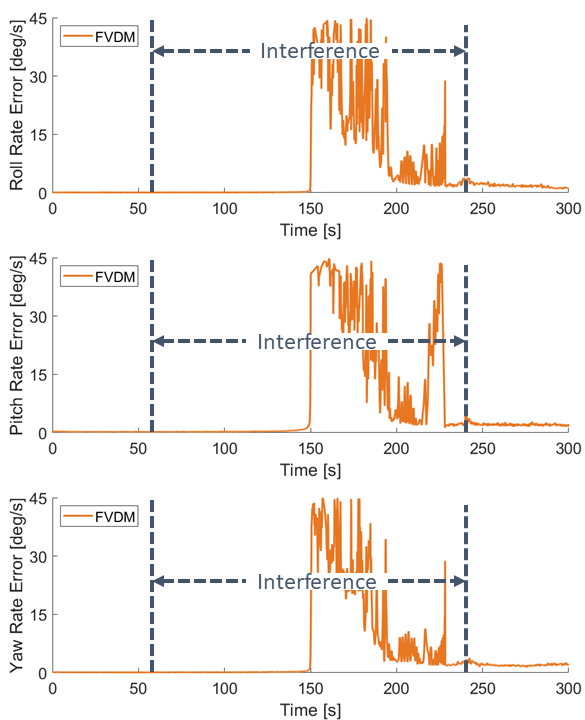
\includegraphics[width=0.75\linewidth]{Figures/Results/trajectoryfigure/Slide13.PNG}
    \caption{Position and speed estimates using the proposed navigation filter when subject to interference that grows stronger as the flight vehicles travels closer to the emitter.}\label{fig:AngScene2}
\end{figure}


\begin{figure}[!ht]
    \centering
    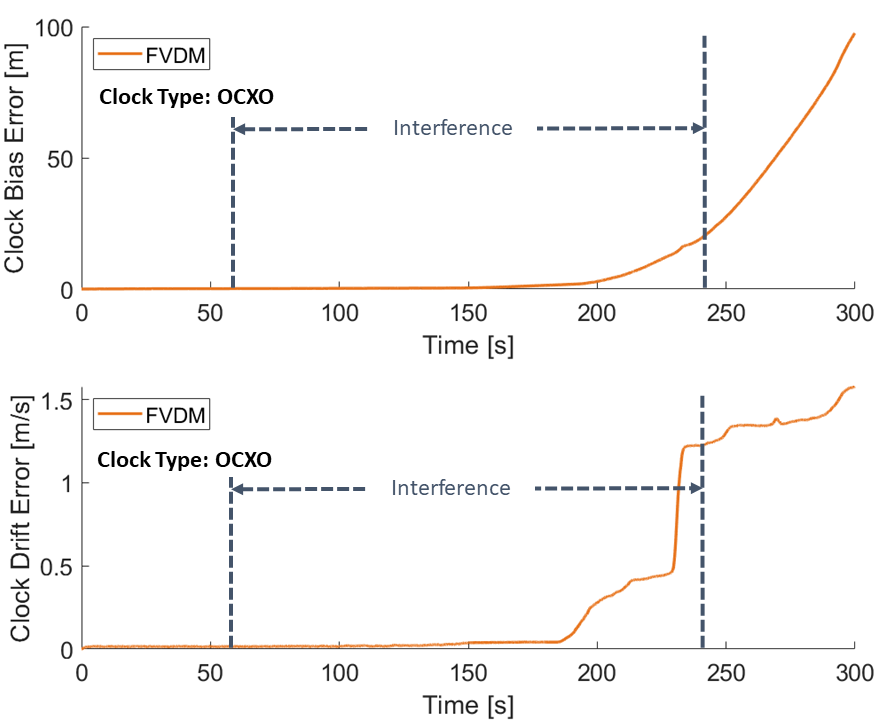
\includegraphics[width=0.75\linewidth]{Figures/Results/trajectoryfigure/Slide25.PNG}
    \caption{Position and speed estimates using the proposed navigation filter when subject to interference that grows stronger as the flight vehicles travels closer to the emitter.}\label{fig:ClkScene2}
\end{figure}


\section{\textbf{Conclusions}}